\documentclass[12pt]{article}

\usepackage{amsmath}
\usepackage{mathtools}
\usepackage{hyperref}
\usepackage{graphicx}
\usepackage{xcolor}
\usepackage{minted}
\usepackage[margin=1.5cm]{geometry}
\usepackage{setspace}
\frenchspacing
\onehalfspace

\usepackage{tikz}
\usetikzlibrary{
	arrows,
	arrows.meta,
	decorations.pathmorphing,
	shapes.multipart
}

\usepackage{helvet}
\renewcommand*{\familydefault}{\sfdefault}

\title{Adding new sources of data}
\author{Benjamin Naecker}
\date{\today}

\begin{document}
\maketitle

\paragraph{Introduction} This document describes the details of the shared library used to 
interact with sources of data (MEAs), and how to add a new data source
when new arrays are acquired. It assumes knowledge of the recording software system,
including details of the \texttt{blds} and the client-server architecture of the system.

\section*{The data source library}

The bulk of the recording programs are written in \texttt{C++}, using the Qt application
framework (see \url{https://qt.io}). The code used to interact with sources of data
is compiled into a shared library called \mintinline{c++}|libdata-source|, which
can be linked to by any executable wanting to talk to the hardware. This usually just
the Baccus lab data server (\texttt{blds}), but could in principle be anything.

\section*{Compiling}

Assuming you have all the dependencies, you can easily compile \texttt{libdata-source}
by opening a terminal, changing to the directory containing the source, and running:

\begin{minted}{bash}
$ qmake
$ make -j release
\end{minted}

\section*{The class hierarchy}

The code for interacting with data sources is desinged as a set of classes. There is
an abstract base class, \mintinline{c++}|BaseSource|, which defines the interface that
all data sources must implement. The current subclasses implement interaction
with the corresponding source of data, shown in the hierarchy in 
figure~\ref{fig.class-hierarchy}.

\begin{figure}
	\centering
	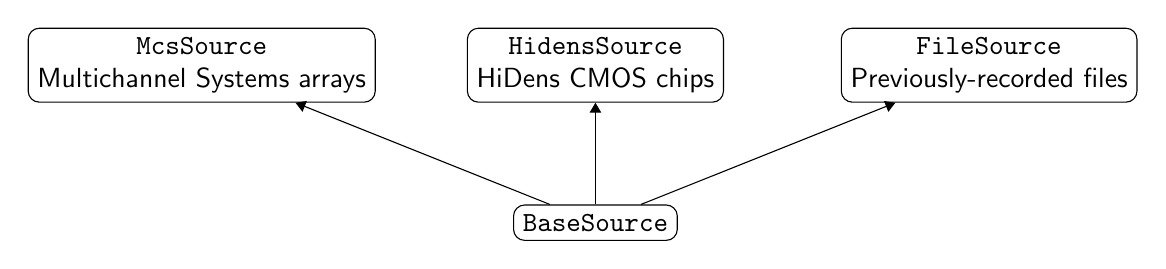
\begin{tikzpicture}
		\node[draw=black,rounded corners] at (5, 0) (base-source) 
			{\texttt{BaseSource}};
		\node[draw=black,rounded corners,align=center] at (0, 2) (mcs-source)
			{\texttt{McsSource} \\
				Multichannel Systems arrays};
		\node[draw=black,rounded corners,align=center] at (5, 2) (hidens-source) 
			{\texttt{HidensSource} \\
				HiDens CMOS chips};
		\node[draw=black,rounded corners,align=center] at (10, 2) (file-source)
			{\texttt{FileSource} \\
				Previously-recorded files};

		\draw[-{Triangle[fill=black]}] (base-source) -> (mcs-source);
		\draw[-{Triangle[fill=black]}] (base-source) -> (hidens-source);
		\draw[-{Triangle[fill=black]}] (base-source) -> (file-source);
	\end{tikzpicture}
	\caption{The data source library class hierarchy.}
	\label{fig.class-hierarchy}
\end{figure}

\section*{The \mintinline{c++}|BaseSource| interface}

This base class describes the interface that any new subclass must implement
in order to be used as a source of data. Data sources follow a very simple state
machine, which defines when operations are valid. The machine is shown in
figure~\ref{fig.state-machine}.

\begin{figure}
	\centering
	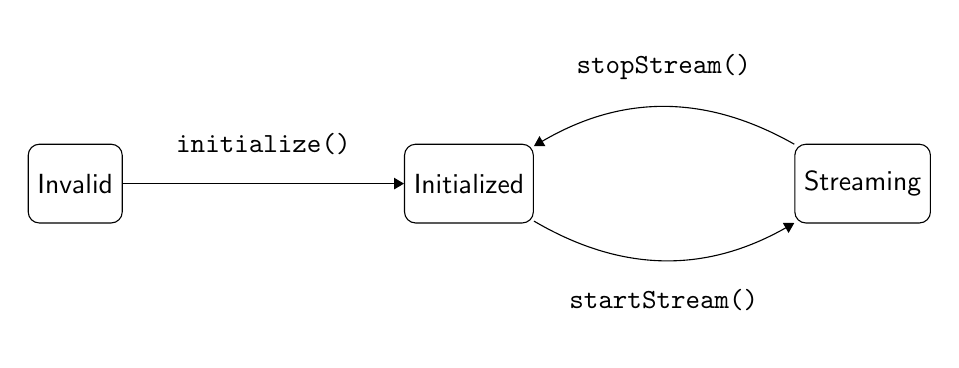
\begin{tikzpicture}[auto,
		node distance=5cm,
		minimum height=1cm,
		bend right]
		\node[draw=black,rounded corners] (invalid) {Invalid};
		\node[draw=black,rounded corners,right of=invalid] (initialized) {Initialized};
		\node[draw=black,rounded corners,right of=initialized] (streaming) {Streaming};

		\draw[-{Triangle[fill=black]}] (invalid) -> (initialized) 
			node[midway] {\texttt{initialize()}};

		\draw[-{Triangle[fill=black]}] (initialized) 
			to node[swap] {\texttt{startStream()}} (streaming);
		\draw[-{Triangle[fill=black]}] (streaming) 
			to node[swap] {\texttt{stopStream()}} (initialized);
	\end{tikzpicture}
	\caption{The data source state machine.}
	\label{fig.state-machine}
\end{figure}

The \texttt{blds} will first try to connect to or create the data source. For the
MCS source, this is just connecting to the NIDAQ device and initializing the driver
library. Next, the \texttt{initialize()} method is automatically called 
(only once), immediately after the data
source object is constructed by \texttt{blds}. Once in the Initialized state, parameters
of the data source may be queried or changed, using a \texttt{get}/\texttt{set} interface.
From the Initialized state, the stream of data may be started or stopped. Once in the
Streaming state, no parameters may be set, but parameter values may still be queried.

\section*{Getting and setting parameters}

The signatures of the \texttt{get()}/\texttt{set()} interface is described below.

\begin{minted}{c++}
class BaseSource {
  /* Constructor and other code */

  /* Request the value of the parameter with name "param" */
  void get(QString param);

  /* Request to set the parameter with name "param" to "value" */
  void set(QString param, QVariant value);
}; // end BaseSource class
\end{minted}

The names of the parameters are just strings (A \texttt{QString} in Qt's type system).
They can be anything, but look at
the file \texttt{include/base-source.h} for the currently-supported parameters.

To make the interface simple, all parameters are set with the same function call.
That is, there is not a \texttt{setGain()}, \texttt{setReadInterval()}, etc method.
Rather, one does:

\begin{minted}{c++}
set("gain", QVariant{5.0});
set("read-interval", QVariant{10});
\end{minted}

\texttt{QVariant} is a Qt class which acts like a type-safe union for a lot of
common data types. That means it can represent pretty much any type of data,
allowing it to be used to set parameters of many different types. It is up to
subclasses to enforce the actual type of the contained object. For example,
for the gain, one probably wants to enforce that this is a double-precision
float, rather than a string or some other type.

\section*{Signals and slots}

You'll notice that the \texttt{get()} call returns \mintinline{c++}|void|.
This is because communication between the \texttt{blds} and data sources happens
via \textit{signals and slots}. These are an integral part of Qt. Signals are
basically notifications of specific types of events, for example, when a timer
expires or new has been written to a file. Slots are just callback
functions. We say that signals are ``emitted'', and slots may be ``connected'' to signals,
meaning that they are called whenever the signal is emitted. This happens
automatically in a Qt application. You only need to worry about connecting
the signals and slots of relevant classes, and Qt will make sure that the slots
are run appropriately.

The reason for doing communication between the \texttt{blds} and sources via
signals and slots is to allow multithreading. Signals and slots allow safe communication
between objects with different thread affinity. That means that the data source
and server can live in different threads, so that the server can be sending data
to any clients at the same time that the source is collecting the newest data.

So, if the \texttt{get()} call returns \mintinline{c++}|void|, 
how do we get information from the source? If you look at the
\mintinline{c++}|BaseSource::get()| member function, you'll see this:

\begin{minted}{c++}
virtual void get(QString param) {
  bool valid = true;
  QVariant data;
  if (param == "trigger") {
      data = m_trigger;
  } else if (param == "state") {
      data = m_state;
  }
  // More conditions, ommitted for brevity
  } else {
      valid = false;
      data = QString{"Unsupported parameter: %1"}.arg(param);
  }
  
  emit getResponse(param, valid, data);
}
\end{minted}

This means that when the \texttt{blds} requests the value of a parameter,
the data source \textit{emits} a response signal with the result. The result
contains the name of the requested parameter, whether or not the parameter
was valid for this source, and, if so, the value encoded as a \mintinline{c++}|QVariant|.
If the requested parameter is not valid, i.e., not supported by this
source, then the variant should contain a helpful error message.

There are signals emitted by the data source like this for each of
the possible transitions in the above state machine. They always contain
a \mintinline{c++}|bool| as one of their arguments, which indicates
whether the request was valid or successful, or not. These signals are:

\begin{minted}{c++}
class BaseSource {
  signals:
    /* Emitted in response to a set() request. */
    setResponse(QString param, bool success, QString msg = {});
  
    /* Emitted in response to a get() request. */
    getResponse(QString param, bool valid, QVariant data = {});
  
    /* Emitted in response to an initialize() request.
     * If the request fails, msg contains an error message.
     */
    initialized(bool success, QString msg = {});
  
    /* Emitted in response to a startStream() request. */
    streamStarted(bool success, QString msg = {});
  
    /* Emitted in response to a stopStream() request. */
    streamStopped(bool success, QString msg = {});
}; // end BaseSource class
\end{minted}

It is up to subclass implementations to decide what constitutes a valid
request. The base class implementation only enforces the state machine, i.e.,
that a \texttt{set()} call in the Streaming state is not allowed.

\section*{Getting data}

The stream of data from a data source can be started and stopped with the
functions \mintinline{c++}|startStream()| and \mintinline{c++}|stopStream()|.
These result in the emission of the \mintinline{c++}|streamStarted()| and
\mintinline{c++}|streamStopped()| signals respectively.

Once the stream has been started, the source should collect data from the
device as soon as possible. (This is part of the reason for putting the
source in its own thread.) The source should then emit the data via a special
signal, with signature:

\begin{minted}{c++}
using Samples = arma::Mat<int16_t>;
void dataAvailable(Samples samples);
\end{minted}

The \texttt{Samples} type is an alias for a matrix of signed 16-bit integers,
using the excellent Armadillo linear algebra library.
This covers the data types represented by both the HiDens and MCS array systems.

This signal is handled by the \texttt{blds} automatically. It writes the
new data to a file and sends it to any clients when they request it. Data
should be collected and emitted in fixed-sized chunks, which defaults to 10
milliseconds of data. (This can be changed in the constructor of the \texttt{BaseSource}
or in the file \texttt{blds.conf}.)

\section*{Example}

Let's make a new class of data source as an example. The source will be incredibly
simple. It will simply emit a new stream of data, where all the values are zeros.

\begin{minted}{c++}
namespace datasource {
class ZeroSource : public BaseSource {
  // Macro required by Qt to deal with signals/slots
  Q_OBJECT

  public:
    ZeroSource() : 
      BaseSource(
      "zero-source" /* source type */,
      "device" /* device type */,
      10 /* read interval, milliseconds */,
      10000.0 /* sample rate, Hz */),
      m_nchannels(100) /* assume we have 100 channels */
      { } // constructor doesn't need to do anything
  
    virtual ~ZeroSource() { } // destructor also doesn't need to do anything
  
  slots:
    /* "Initializing" the source is just filling the chunk of data
     * to be sent to the blds with zeros.
     */
    virtual void initialize() override
    {
      m_dataChunk.set_size(frameSize, m_nchannels);
      m_dataChunk.fill(0);
    }
    
    /* Starting the stream is just setting up a timer
     * on which to send data.
     */
    virtual void startStream() override
    {
      /* Enforces the state machine. */
      BaseSource::startStream();
    
      /* Timer will fire every 10ms, at which point we'll send the
       * chunk of zeros to the blds.
       */
      m_timer.setInterval(m_readInterval);
      QObject::connect(&m_timer, &QTimer::timeout, this, &ZeroSource::sendData);
      m_timer.start();
    }
    
    /* Stopping the stream is just stopping the timer. */
    virtual void stopStream() override
    {
      BaseSource::stopStream();
      m_timer.stop();
    }
    
    /* Setting any parameter is disallowed in this example. */
    virtual void set(QString param, QVariant /* unused */)
    {
      emit setResponse(param, false, "Cannot set parameters of a ZeroSource.");
    }

  private:
    /* Handler function which sends data to the blds. */
    void sendData()
    {
      emit dataAvailable(m_dataFrame);
    }
    
    /* The frame of data to send to the blds. */
    Samples m_dataFrame;
    
    /* Timer used to simulate acquisition of new data. */
    QTimer m_timer;
    	  
}; // end ZeroSource class
}; // end datasource namespace
\end{minted}

So to summarize, all this simple source does is send the \texttt{blds} a chunk
of 100 samples of zeros for each of the 100 channels, every 10 milliseconds. After
recompiling \texttt{libdata-source}, you have to make sure that \texttt{blds}
is re-linked with this new version of the library. On Linux or MacOS, you don't really
need to do anything. These systems link executables with a ``versionless''
library, e.g., \texttt{libdata-source.so}, which is usually a symbolic link
to the latest version of the library. That means the dynamic loader will
find the new version.

Windows is insane when it comes to shared libraries. The best thing to do is
re-compile \texttt{libdata-source}, and then literally copy the new library into
the directory containing the \texttt{blds} executable.

\end{document}
